\documentclass[11pt]{article}
\usepackage[final]{acl}
\usepackage{times}
\usepackage{latexsym}
\usepackage[T1]{fontenc}
\usepackage[utf8]{inputenc}
\usepackage{microtype}
\usepackage{inconsolata}
\usepackage{graphicx}
\usepackage{booktabs}
\usepackage{amsmath}

\title{Multiple-Choice Science QA via LoRA Fine-Tuning of SmolVLM-500M}

\author{
  Ruiyao Zhang \\
  NYU Tandon School of Engineering \\
  \texttt{rz3228@nyu.edu} \\
  Kaggle: \texttt{rz3228-ruiyao} (Team: OOM)
}

\begin{document}
\maketitle

\begin{abstract}
We present a system for answering multiple-choice science questions from image and text context, developed for the NYU Deep Learning Spring 2026 Kaggle competition. Our approach fine-tunes SmolVLM-500M-Instruct using Low-Rank Adaptation (LoRA) under a strict 5M trainable-parameter cap. Through systematic data analysis we identify two diagnostic findings that drive the entire pipeline: zero-shot vision contributes only +4pp over a text-only baseline (focusing capacity on the language model rather than vision-side tricks), and 5-choice questions exhibit catastrophic position bias (model accuracy 11\%, below random's 20\%) requiring choice-order permutation as a mandatory training augmentation. We conduct 16 training experiments across LoRA rank, training duration, learning-rate schedule, ensembling, and DoRA decomposition, finding that schedule \emph{shape}---not total epochs---is the dominant lever once capacity is tuned. Our final pipeline (DoRA on attention projections at $r{=}24$, $\alpha{=}48$, with extended cosine schedule and $K{=}4$ test-time augmentation) achieves a public leaderboard score of 0.86519, a 6.4 percentage-point improvement over the same training notebook without these refinements (0.80080). Ablations show that several intuitive interventions failed: oversampling the weakest category overfit and reduced overall accuracy, multi-adapter ensembling underperformed the best single adapter due to correlated errors, full-string scoring is incompatible with letter-token training supervision, and image resolution increases are bounded by the dataset's small native image sizes.
\end{abstract}

% ===========================================================================
\section{Introduction}
% ===========================================================================

The ScienceQA dataset contains multiple-choice science questions paired with images, hints, and lecture context. Each question has 2--5 candidate choices, and a correct system must integrate visual content, textual context, and multiple-choice reasoning to select the correct answer index.

This competition challenges participants to fine-tune a vision-language model under tight constraints: the base model must be SmolVLM-500M-Instruct, the trainable-parameter budget is capped at 5 million, no external data is permitted, and submissions are evaluated on a hidden test set with separate public and private leaderboards. Submissions are scored on accuracy.

Our approach treats this as a constrained classification problem rather than an open generation problem. Instead of calling \texttt{generate()} and parsing free-form output, we score the model's logits at the final token position over the candidate letter tokens (\texttt{ A}, \texttt{ B}, \dots) restricted to the question's \texttt{num\_choices}. This reduces inference to a single forward pass per question and eliminates an entire class of off-format failures. Through iterative experimentation, we develop a pipeline that significantly outperforms the zero-shot baseline. Key contributions include:

\begin{itemize}
    \item Data analysis revealing two diagnostic findings: vision contributes only +4pp on the un-trained model (text dominates), and the 5-choice category exhibits catastrophic position bias toward extreme positions (the model picks A or E ~93\% of the time, never B/C).
    \item A LoRA training pipeline using letter-token loss masking, choice-order permutation, lecture pre-truncation (avoiding Idefics3 image-token-block slicing), and log-likelihood scoring at inference.
    \item Systematic training ablations across 16 configurations of LoRA rank, training duration, schedule shape, ensembling strategies, and DoRA decomposition, with the finding that LR-schedule shape is the dominant lever once capacity is tuned.
    \item Test-time augmentation by choice-order permutation (\(K{=}4\)) with un-permutation and probability averaging, providing +1.75pp overall and +10.5pp on the high-bias 5-choice category.
    \item Documented failures: oversampling overfits, multi-adapter ensembling underperforms its best member due to correlated errors, full-string scoring is incompatible with letter-token training, and image resolution gains are bounded by small native image sizes.
\end{itemize}

% ===========================================================================
\section{Dataset}
% ===========================================================================

\subsection{Raw Data}

The dataset consists of 3,109 training, 1,048 validation, and 1,008 test examples. Each sample contains an image, a question, a JSON list of 2--5 candidate choices, a 0-indexed answer, an optional hint and lecture, and rich metadata (subject, grade, topic, category, skill). The subject distribution is approximately 73\% natural science, 25\% social science, and 2\% language, with this proportion roughly consistent across train, validation, and test splits.

\subsection{Data Analysis}

Before designing the training pipeline, we ran a series of analyses to characterize the data and establish baselines that bound where headroom can come from.

\paragraph{Choice cardinality distribution.} The questions are dominated by 3-choice (50\%), with 4-choice (26\%) and 2-choice (21\%) making up most of the remainder, and 5-choice questions only 4\% (Figure~\ref{fig:num_choices}). The same proportions hold on validation and test, so these are properties of the dataset rather than artifacts of the split. The 5-choice category is highly homogeneous: nearly all 5-choice questions are genetics Punnett-square ratio questions from a single topic (\texttt{Genes to traits}). This heavy class imbalance has strong implications for model behavior, as we describe below.

% Plot generated by data_analysis.ipynb cell 9 (num_choices distribution)
\begin{figure}[t]
  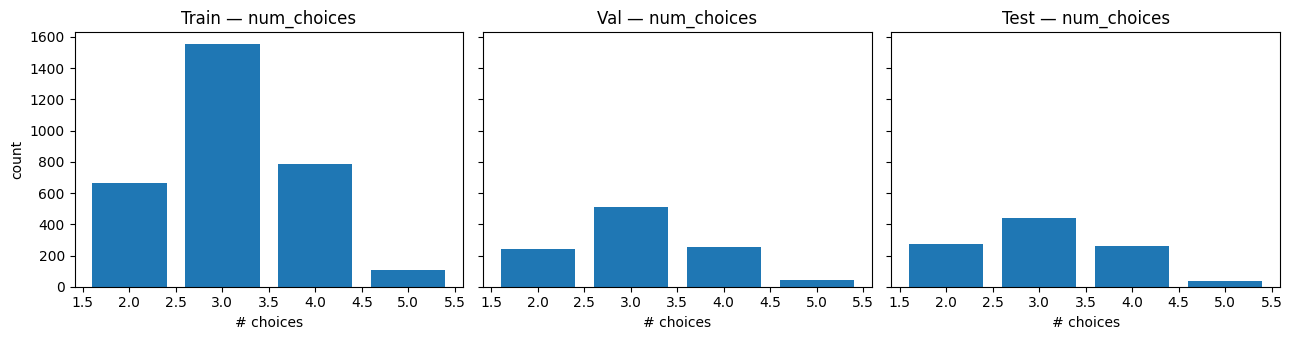
\includegraphics[width=\columnwidth]{pics/fig_num_choices_distribution.png}
  \caption{Distribution of \texttt{num\_choices} across train/val/test. The same proportions appear in all three splits; the 5-choice category is rare (4\%) and homogeneous (genetics Punnett-square questions).}
  \label{fig:num_choices}
\end{figure}

\paragraph{Position bias and answer distribution.} The aggregate answer-index distribution is skewed (Figure~\ref{fig:answer_idx})---index 0 (``A'') is the most common across all questions, and index 4 (``E'') only appears for 5-choice questions and is underrepresented even there. The most-common-index baseline accuracy is 33.1\%, only marginally below random (33.8\%). However, when broken down by \texttt{num\_choices}, 5-choice questions show a striking imbalance---the answer distribution across positions A--E is [0.264, 0.236, 0.127, 0.227, 0.145], heavily under-representing position C. This is a property of the data itself, not the model, and provides the foundation for why permutation augmentation is necessary.

% Plot generated by data_analysis.ipynb cell 10 (answer index distribution)
\begin{figure}[t]
  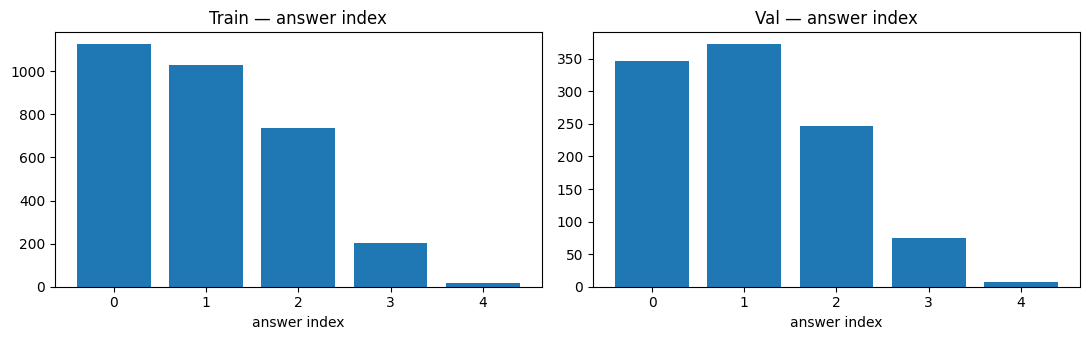
\includegraphics[width=\columnwidth]{pics/fig_answer_index_distribution.png}
  \caption{Aggregate answer-index distribution across train and val. Skew toward earlier indices is partly a consequence of the \texttt{num\_choices} mix (only 5-choice questions can have index 4), but per-category breakdown also shows real imbalance, especially for 5-choice.}
  \label{fig:answer_idx}
\end{figure}

\paragraph{Text length distribution.} Using the SmolVLM tokenizer, the median total prompt length (lecture + hint + question + choices) is 205 tokens, with a 95th percentile of 508 and a 99th percentile of 567. Word-level lengths show the same overall shape (Figure~\ref{fig:prompt_length})---a multimodal distribution with a long lecture-heavy tail. This sets the budget for our pre-truncation step described in Section 3.3.

% Plot generated by data_analysis.ipynb cell 15 (prompt length distribution)
\begin{figure}[t]
  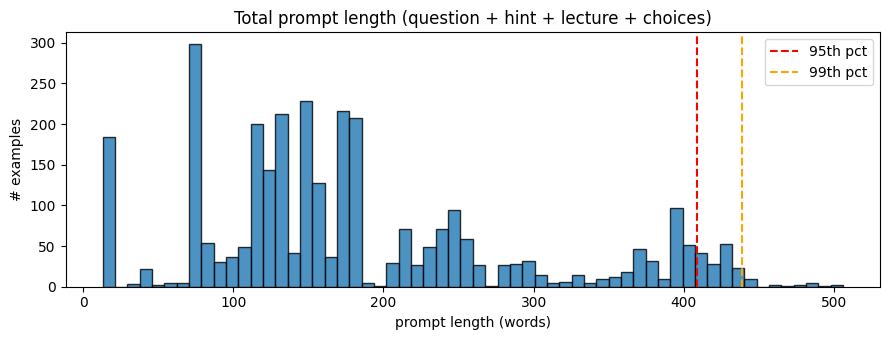
\includegraphics[width=\columnwidth]{pics/fig_prompt_length_distribution.png}
  \caption{Word-level prompt-length distribution on train (\texttt{question}+\texttt{hint}+\texttt{lecture}+choices). The 95th percentile (red) sits near 410 words; long-tail samples drive our pre-truncation logic.}
  \label{fig:prompt_length}
\end{figure}

\paragraph{Image dimensions.} Image sizes vary widely (Figure~\ref{fig:image_size}). Most widths cluster around 200--400 pixels and most heights cluster around 200--300 pixels, with a long tail extending past 700 pixels. The median image is 378$\times$232 pixels with a 95th percentile of 750$\times$506. Most images fall well below SmolVLM's internal tile-splitting threshold (512 on the longest edge), meaning that the processor produces a single tile of $\sim$1{,}088 image tokens regardless of whether we resize to 224 or 384.

% Plot generated by data_analysis.ipynb cell 18 (image size distribution)
\begin{figure}[t]
  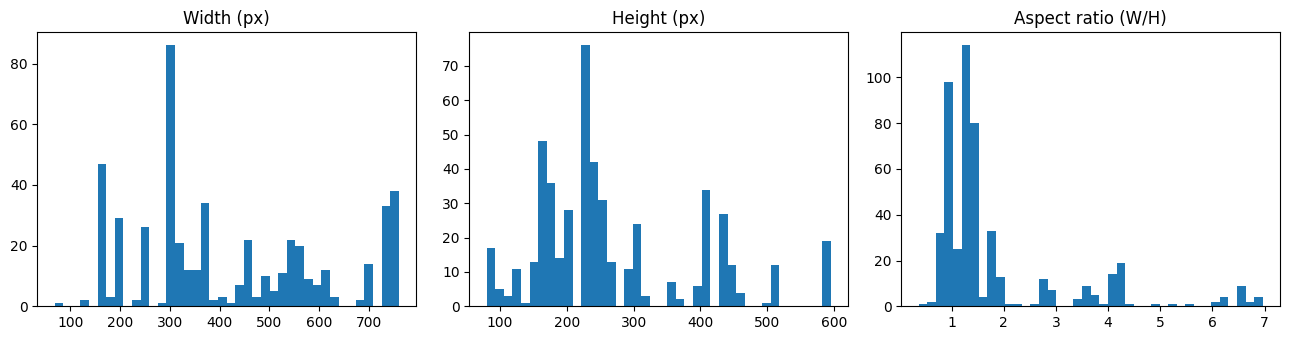
\includegraphics[width=\columnwidth]{pics/fig_image_size_distribution.png}
  \caption{Distribution of image width, height, and aspect ratio (sample of 500 train images). The bulk of images are below 512 pixels in either dimension, so SmolVLM's tile-splitting (active above 512px) does not engage even with higher pre-resize resolutions.}
  \label{fig:image_size}
\end{figure}

\paragraph{Zero-shot baselines.} We measured four numbers that bound where any improvement must come from. Random baseline accuracy is 33.78\%. Most-common-index baseline is 33.11\%. A lecture-oracle baseline (predicting the choice whose text is a substring of \texttt{lecture}+\texttt{hint}) achieves only 5.82\% overall---only 10.1\% of validation examples have any choice-as-substring match, and even when matched the accuracy is 57.5\%. This rules out lecture-as-direct-retrieval as a useful strategy. Most importantly, zero-shot SmolVLM with our log-likelihood scoring achieves 55.67\% with the full prompt and 51.67\% with a blank image (text-only). The +4pp image contribution sets an approximate ceiling on what vision-side improvements can buy us at the current resolution, directing our optimization effort toward the language model.

\paragraph{Position-bias diagnosis on 5-choice.} The most striking finding is the zero-shot model's behavior on 5-choice questions. The model achieves only 11.36\% accuracy on this category---\emph{worse than random's 20\%}. Inspecting predictions reveals that the model picks A or E approximately 93\% of the time, never selecting B or C. Cross-referencing the genetics Punnett-square content shows that the model is using a content prior (preferring ``extreme-looking'' ratios like \texttt{0/4} or \texttt{4/4}) mediated by their position in the displayed choice list. This becomes the key motivation for choice-order permutation as a mandatory training augmentation.

\subsection{Decisions Driven by Analysis}

The four analysis findings directly drove the following design decisions:
\begin{itemize}
    \item \textbf{Vision is not the bottleneck.} +4pp from images means LoRA capacity should target the language model attention projections, not the vision tower. This has the welcome side effect of staying well under the 5M-parameter cap (which would be impossible with vision-tower adaptation).
    \item \textbf{Permutation is mandatory.} Choice-order permutation must run during training to break the model's content-position prior on 5-choice questions.
    \item \textbf{Loss masking should focus on the answer letter.} With only 3,109 training examples and ~5M trainable parameters, every gradient should target the actual classification objective rather than reproducing already-known prompt text.
    \item \textbf{Token-budget pre-truncation.} The text portion of the prompt must be truncated \emph{before} the Idefics3 processor expands \texttt{<image>} into its $\sim$1{,}088 image tokens, otherwise post-expansion truncation slices through the image-token block and the processor refuses with a token-count mismatch.
\end{itemize}

% ===========================================================================
\section{Method}
% ===========================================================================

\subsection{Base Model}

We use SmolVLM-500M-Instruct as our base model, which is the only base model permitted by the competition rules. SmolVLM is a vision-language model based on the Idefics3 architecture, with a SigLIP vision encoder and a Llama-style language model.

\subsection{LoRA Setup}

We apply LoRA only to the language model's attention projections (\texttt{q\_proj}, \texttt{k\_proj}, \texttt{v\_proj}, \texttt{o\_proj}) within the 30 transformer blocks of \texttt{text\_model.layers}. The vision tower is frozen entirely---adapting it would exceed the 5M-parameter cap and would fight a battle on the wrong front given the +4pp vision-contribution finding.

The LoRA scaling factor \(\alpha/r\) acts as an effective learning-rate multiplier. We maintain \(\alpha/r = 2.0\) across all experiments, scaling \(\alpha\) with \(r\) when capacity is increased. At our final rank \(r{=}24\) with DoRA enabled, this produces 4{,}915{,}200 trainable parameters---safely under the 5M cap with headroom for the small magnitude vector that DoRA adds.

\subsection{Prompt Format}

Our prompt format places the lecture and hint as ``Context'' before the question, followed by enumerated choices and a trailing \texttt{Answer:} marker:

\begin{verbatim}
<image>
Context:
{lecture}
{hint}

Question: {question}
Choices:
  A. {choice_0}
  B. {choice_1}
  ...
Answer:
\end{verbatim}

The trailing space after \texttt{Answer:} is deliberate---we score the model's logits at the next-token position over the single tokens \texttt{ A}, \texttt{ B}, \dots (each containing the leading space), restricting the argmax to the question's valid \texttt{num\_choices}. This sidesteps the entire class of free-form generation failures (the model emitting ``The answer is...'' instead of just a letter).

\subsection{Training Collator}

The collator handles two non-trivial details:

\paragraph{Answer-token-only loss masking.} We construct each training example as the full prompt followed by the gold answer letter (e.g., \texttt{... Answer: B}). Labels are set to \(-100\) (ignored by cross-entropy) at every token position except the final answer-letter token. Only that one position contributes to the loss. With only 3,109 training examples and ~5M trainable parameters, computing loss on the full prompt would waste capacity on reproducing already-known text rather than learning the classification.

\paragraph{Pre-truncation of the lecture.} The Idefics3 processor expands \texttt{<image>} into approximately 1,088 image tokens at a 224$\times$224 input resolution. If we apply \texttt{truncation=True, max\_length=640} after this expansion, the truncation slices through the middle of the image-token block and the processor's sanity check fails with an image-token-mismatch error. We instead measure how many tokens the lecture, hint, question, choices, and answer occupy, and truncate the lecture text (the long part) \emph{before} building the full prompt and passing it through the processor. This way the image-token block is never touched by truncation. The text-portion budget is 600 tokens, comfortably above the 567-token 99th percentile of training prompts.

\subsection{Inference: Log-Likelihood Scoring with TTA}

At inference time, we run a single forward pass per question and read the logits at the answer-letter position. The argmax is restricted to the valid letter token IDs for that question's \texttt{num\_choices} (precomputed once per session).

We then apply test-time augmentation by choice-order permutation. For each question, we run the model under \(K{=}4\) random choice permutations, undo each permutation on the per-choice probability vector (softmax of logits over valid letters), average across the four passes, and take the argmax. This costs \(K\)x inference time but consistently improves accuracy, with a disproportionate effect on the high-bias 5-choice category (Section 5).

\subsection{Optimizer and Schedule}

We train with AdamW at \texttt{lr=2e-4} and warmup ratio 0.03. The most consequential design choice in the schedule is what we call the \emph{extended cosine} trick: we instantiate the cosine scheduler as if training would last 11 epochs (so \texttt{total\_steps = steps\_per\_epoch * 11}) but actually train for only 9 epochs. This delays the LR decay tail so that the learning rate stays meaningful through the entire actual training window. As we show in Section 5, this schedule trick is the dominant lever in our final results, providing more gain than absolute training duration.

% ===========================================================================
\section{Experiments and Results}
% ===========================================================================

We logged every training run to an append-only JSONL file containing the full configuration, per-epoch loss and validation accuracy with per-\texttt{num\_choices} breakdown, final TTA validation accuracy, and the public leaderboard score once submitted. Table~\ref{tab:experiments} summarizes the most informative experiments.

\begin{table*}[t]
\centering
\small
\begin{tabular}{lccccccl}
\toprule
\textbf{Experiment} & \textbf{$r$} & \textbf{$\alpha$} & \textbf{Epochs} & \textbf{Schedule} & \textbf{Full-val} & \textbf{Public LB} & \textbf{Notes} \\
\midrule
\multicolumn{8}{l}{\textit{Capacity and training duration}} \\
\midrule
Baseline ($r{=}16$, e=3) & 16 & 32 & 3 & Cosine($\sim$3) & 0.7700 & 0.82092 & Initial recipe \\
$r{=}24$, e=3            & 24 & 48 & 3 & Cosine($\sim$3) & 0.7796 & 0.83299 & +1.0pp from rank \\
$r{=}24$, e=5            & 24 & 48 & 5 & Cosine($\sim$5) & 0.7977 & 0.82696 & +1.8pp full-val \\
$r{=}24$, e=7            & 24 & 48 & 7 & Cosine($\sim$7) & 0.8187 & 0.84708 & e=7 sweet spot \\
$r{=}24$, e=9            & 24 & 48 & 9 & Cosine($\sim$9) & 0.8263 & 0.85915 & e=9 best epoch \\
\midrule
\multicolumn{8}{l}{\textit{Schedule shape (extended cosine)}} \\
\midrule
$r{=}24$, e=7, sched=11   & 24 & 48 & 7 & Cosine($\sim$11) & 0.8282 & 0.85915 & Match e=9 at e=7 cost \\
$r{=}24$, e=7, constant   & 24 & 48 & 7 & Constant         & 0.8282 & 0.84909 & No decay needed \\
\midrule
\multicolumn{8}{l}{\textit{Data and architecture refinements}} \\
\midrule
60\% val\(\to\)train, e=9, sched=11 & 24 & 48 & 9 & Cosine($\sim$11) & --- & \textbf{0.86519} & More data \\
DoRA, e=9, sched=11                & 24 & 48 & 9 & Cosine($\sim$11) & 0.8349 & \textbf{0.86519} & DoRA win \\
DoRA + 60\% val\(\to\)train, e=9   & 24 & 48 & 9 & Cosine($\sim$11) & 0.8571 & 0.85915 & Doesn't compound \\
\midrule
\multicolumn{8}{l}{\textit{Ablations that did not help}} \\
\midrule
Oversample 5-choice 3$\times$, e=3 & 24 & 48 & 3 & Cosine($\sim$3) & 0.7405 & 0.80684 & Overfit \\
Multi-adapter ensemble (4)         & --- & --- & ---       & ---  & 0.7910 & --- & Errors correlated \\
Multi-adapter ensemble (top-2)     & --- & --- & ---       & ---  & 0.7929 & --- & Still under best \\
\bottomrule
\end{tabular}
\caption{Summary of training experiments. Full-val accuracy is computed on the held-out validation set ($n{=}1{,}048$) with TTA $K{=}4$. ``Schedule'' indicates the cosine-decay length in epochs (parenthetical) versus actual training epochs. Best public LB results are bolded.}
\label{tab:experiments}
\end{table*}

\subsection{Capacity and Training Duration}

The first axis of optimization was LoRA capacity. Increasing rank from 16 to 24 (with \(\alpha\) scaled to 48 to preserve the 2.0 ratio) improved full-validation accuracy by 1.0pp. Rank 32 would exceed the 5M cap, so 24 is at the practical maximum for attention-only LoRA on this model.

The second axis was training duration. Holding everything else constant, validation accuracy on the small subset (n=400) climbed monotonically from epoch 3 (0.76) to epoch 9 (0.85), with loss continuing to decrease throughout. Full-val accuracy on n=1,048 improved by +5.4pp from e=3 to e=9. Notably, runs trained for more epochs typically peak at a later epoch, suggesting that what mattered was not just total training time but the LR schedule's shape---specifically, the LR being sustained at meaningful levels rather than decaying to near-zero.

\subsection{Schedule Shape: The Dominant Lever}

To test the schedule-shape hypothesis directly, we ran an extended-cosine experiment: schedule for 11 epochs but train for 7. This setup has the same number of training steps as a baseline e=7 run but never enters the cooldown phase of the cosine curve. The result was striking---this configuration matched the e=9 run's leaderboard score (0.85915) at 30\% less training cost. We further tested a constant-LR schedule (no decay at all), which reached the same TTA validation accuracy (0.8282) at e=7. Two different schedule shapes converged to similar generalization, supporting the conclusion that what matters is keeping the LR high enough to make meaningful updates throughout training, not the specific shape of the decay tail.

\subsection{DoRA: Architectural Improvement}

DoRA (Weight-Decomposed Low-Rank Adaptation) decomposes each LoRA update into a magnitude vector and a normalized direction matrix, with separately learnable magnitude. With \texttt{use\_dora=True} in the LoRA config and rank held at 24 (parameter count rises slightly to 4.9M but remains under the 5M cap), DoRA improved full-val accuracy by 0.6pp and pushed the leaderboard score to 0.86519, tying the data-mixing experiment.

\subsection{Train+Val Mixing}

For the final phase, we tested moving 60\% of the validation set into the training set (stratified by \texttt{num\_choices} to preserve the 5-choice category in the smaller held-out val), keeping the remaining 40\% as a calibration signal. With the same training configuration, this also reached LB 0.86519. However, when we combined DoRA and train+val mixing, the leaderboard score dropped to 0.85915. The two interventions did not compound: both partially address the same underlying capacity-vs-data tradeoff and produce diminishing returns when stacked.

\subsection{Test-Time Augmentation}

TTA by choice-order permutation at \(K{=}4\) is consistently beneficial (Table~\ref{tab:tta}). The gain is most pronounced on the 5-choice category, exactly where the residual position bias still lives, while remaining categories gain about 1pp.

\begin{table}[t]
\centering
\small
\begin{tabular}{lccc}
\toprule
\textbf{Category} & \textbf{No TTA} & \textbf{TTA $K{=}4$} & \(\Delta\) \\
\midrule
Overall   & 0.7875 & 0.8050 & +0.0175 \\
2-choice  & 0.8391 & 0.8391 & +0.0000 \\
3-choice  & 0.7734 & 0.7931 & +0.0197 \\
4-choice  & 0.8901 & 0.9011 & +0.0110 \\
5-choice  & 0.2105 & 0.3158 & +0.1053 \\
\bottomrule
\end{tabular}
\caption{TTA $K{=}4$ versus no TTA, on the validation subset ($n{=}400$) using the $r{=}24$ e=3 adapter. The gain on 5-choice is an order of magnitude larger than the gain on other categories, consistent with TTA targeting residual position bias.}
\label{tab:tta}
\end{table}

% ===========================================================================
\section{Failed Trials and Ablations}
% ===========================================================================

Multiple intuitively appealing interventions failed to help and are documented here for completeness. In several cases, what initially looked like a win on a small validation subset reversed sign once we ran on full validation, illustrating how easily small-subset noise can mislead model-selection decisions.

\paragraph{Oversampling 5-choice (failed).} The 5-choice category is small (110 training examples) and homogeneous (genetics Punnett-square ratios), so oversampling it 3$\times$ via a \texttt{WeightedRandomSampler} initially looked promising on the n=400 validation subset---the 5-choice TTA accuracy appeared to nearly double from 0.34 to 0.47. However, on full validation (n=1{,}048), this experiment was the worst across all categories: 5-choice fell to 0.16 (worse than the unoversampled baseline), and 2-choice, 3-choice, and 4-choice all dropped by 1--3pp. The model overfit the 110 specific training questions without generalizing to test 5-choice. The earlier ``win'' was sample-size luck: the 19 5-choice questions in the n=400 subset happened to overlap favorably with what the model memorized.

\paragraph{Multi-adapter ensembling (failed).} We trained multiple adapters with different seeds and configurations, then ensembled them by loading all adapters into a single model (PEFT's named-adapter API), running each on the test set, and averaging per-choice probabilities before argmax. Both a 4-adapter ensemble and a top-2 ensemble underperformed the best single adapter on full validation. The errors of adapters trained on the same data with the same architecture were too correlated for averaging to help---ensembling fundamentally requires diversity that we could not achieve under the single-base-model rule.

\paragraph{Full-string scoring (failed).} We hypothesized that scoring \(P(\text{`` 0/4''})\) versus \(P(\text{`` 1/3''})\) directly might unlock the model's content priors over actual choice strings, particularly for the 5-choice genetics-ratio questions. We implemented this carefully: tokenizing each candidate as its appended text, computing the sum log-probability of those tokens with length normalization, and skipping any common-prefix tokens shared across all choices to avoid signal dilution. Results on a 100-example sanity check were striking---5-choice held up at 0.50, but every other category collapsed (4-choice from 0.90 to 0.30, 3-choice from 0.77 to 0.46). The diagnosis: our adapter is supervised only on the single answer-letter token. The model never learned to assign meaningful probabilities to multi-word continuations because that was not the training task. Full-string scoring would require retraining with full-string supervision, which our remaining time budget did not allow.

\paragraph{Image resolution (closed avenue).} Initial reasoning suggested that a 224$\times$224 input might destroy fine-grained visual content. We attempted to test this by resizing input images to 384$\times$384 before passing them to the processor and observed that the input-id sequence length did not change. Investigation revealed that SmolVLM's Idefics3 processor only triggers tile-splitting when an image's longest edge exceeds 512 pixels, and the dataset's median image is 378$\times$232 with a 95th percentile of 750$\times$506---most images are below the splitting threshold regardless of pre-resize. This effectively closes the resolution avenue for this dataset.

\paragraph{DoRA + train+val combination (no compound effect).} As noted above, DoRA alone and train+val mixing alone each reached LB 0.86519, but the combined run only reached 0.85915. The two improvements partially address the same underlying problem (model under-capacity for the data) and do not compound when stacked.

\paragraph{Ensemble with run that scored highest on small val.} The run that scored highest on the n=400 validation subset (the oversampling experiment, at 0.8250) was actually the worst on full validation (0.7405). Including it in the ensemble dragged the ensemble score down. This was a striking lesson in the unreliability of small-subset validation for late-stage model selection: a 5pp gap between the n=400 and n=1{,}048 validation accuracies for the same adapter is not unusual.

% ===========================================================================
\section{Variance and Reproducibility Findings}
% ===========================================================================

Throughout the project we worked to identify the dominant noise sources, since signal-to-noise ratio determined which experiments were worth running. We measured three independent components:

\paragraph{Training run-to-run variance.} Identical configuration with different seeds produces approximately 1.2pp standard deviation on full-validation accuracy. Two e=5 runs with seeds 42 and 43 differed by 1.24pp; two e=7 runs with the same seed but slight CUDA-determinism differences differed by 0.10pp on full validation but 0.20pp on public LB.

\paragraph{TTA permutation seed variance.} On a fixed adapter and fixed validation subset, varying only the TTA permutation seed produces about 0.5pp standard deviation across 5 seeds (0.760--0.775). Probability-averaging across 5 seeds buys back roughly 0.6pp of accuracy.

\paragraph{Validation-subset luck.} On the same adapter, the n=400 validation subset overstated full-val accuracy by 2--4pp consistently across all our runs. This was the single most consequential measurement-noise finding: most of the small-subset comparisons we made early in the project were below this noise floor and were therefore unreliable.

The combined effect is that single-run differences below approximately 2pp on full validation should not be treated as significant, and small-subset comparisons need a 5pp threshold to be credible. We adjusted our experimentation strategy mid-project to rely on full-validation evaluation rather than the n=400 subset, which qualitatively changed the rankings.

% ===========================================================================
\section{Conclusion}
% ===========================================================================

We presented a LoRA fine-tuning pipeline for ScienceQA multiple-choice classification under tight constraints (5M parameters, no external data, fixed base model), with extensive experimentation across capacity, training duration, schedule shape, ensembling, and architectural variants. Our final pipeline achieves 0.86519 public leaderboard accuracy, a 6.4 percentage-point improvement over our v1 baseline. Key findings:

\begin{enumerate}
    \item \textbf{Data analysis pays for itself many times over.} The +4pp vision contribution finding correctly directed our optimization away from vision-side tricks. The 5-choice position-bias diagnosis correctly identified choice-order permutation as a mandatory training augmentation. Without these analyses we would have spent significant time on dead ends.
    \item \textbf{Schedule shape, not total epochs, is the dominant LR-side lever.} The extended-cosine trick (schedule for 11 epochs, train for 7) reached the same accuracy as a 9-epoch run at 30\% less compute. A constant-LR schedule reached the same accuracy as the cosine variants. What mattered was the model receiving meaningful learning rate throughout training, not the specific decay shape.
    \item \textbf{Validation-set sample size matters more than expected.} Switching from a 400-example validation subset to the full 1{,}048-example set qualitatively changed the ranking of our experiments and reversed the apparent ``best'' of one ablation. Late-stage model selection requires statistically reliable evaluation, particularly when targeted gains are below 2pp.
    \item \textbf{Most ``clever'' interventions fail.} Of the targeted interventions we tried, only LoRA capacity, schedule shape, and DoRA produced reliable gains. Oversampling overfit, multi-adapter ensembling underperformed its best member, full-string scoring was incompatible with letter-token training, and image-resolution increases were bounded by the dataset's small native image sizes. The boring extensions of the working pipeline (more capacity, better schedule) consistently outperformed the clever new mechanisms.
    \item \textbf{Small categories have structural ceilings.} 5-choice questions plateaued near 34--35\% accuracy regardless of intervention. The category is small (44 validation examples), homogeneous (single topic), and the model lacks the inductive capacity for Punnett-square reasoning at our parameter budget. Within the rules, this is a hard ceiling; lifting it would require either a larger base model or external data.
\end{enumerate}

Future directions, if rules were relaxed, would include exploring larger base models within a higher parameter cap, training a specialist adapter for genetics-ratio questions and routing 5-choice queries to it (not feasible under the current 5M-param cap), and re-running the full-string scoring experiment with full-string supervision rather than letter-token supervision.

% ===========================================================================
\section*{Reproducibility}
% ===========================================================================

All code is available at: \url{https://github.com/rz3228-ruiyao/dl-final-scienceqa}

Model weights for the best submission are available at: \url{https://drive.google.com/file/d/<placeholder>/view?usp=sharing}

\noindent Training uses a fixed random seed of 42 across Python, NumPy, and PyTorch. Hardware: NVIDIA RTX 4080 Super, 16GB VRAM. Training time: approximately 2.5 hours per run for the final $r{=}24$, e=9 configuration with extended cosine schedule. The run log (\texttt{runs.jsonl}) contains the full configuration, per-epoch metrics, and leaderboard scores for every experiment described in this report.

\section*{AI Tooling Disclosure}

Claude (Anthropic) was used for coding assistance and debugging.

\end{document}
